\documentclass[12pt,letterpaper]{article}

\usepackage[utf8]{inputenc}
\usepackage[T1]{fontenc}
\usepackage[spanish]{babel}
\usepackage[margin=2.5cm]{geometry}
\usepackage{graphicx}
\usepackage{booktabs}
\usepackage{array}
\usepackage{caption}
\usepackage{hyperref}
\usepackage{xcolor}
\usepackage{listings}
\usepackage{float}

\hypersetup{
    colorlinks=true,
    linkcolor=blue,
    filecolor=blue,
    urlcolor=blue
}

% Configuración de las figuras
\captionsetup[figure]{font=small,labelformat=simple,labelsep=period}
\captionsetup[table]{font=small,labelformat=simple,labelsep=period}

% Renombrar "Figura" y "Tabla" a español
\renewcommand{\figurename}{Figura}
\renewcommand{\tablename}{Tabla}

\title{}
\author{}
\date{}

\begin{document}

\begin{titlepage}
    \centering
    \vspace*{2cm}

    {\Large\bfseries Computación de Alto Rendimiento (HPC)\par}
    \vspace{0.5cm}
    {\Large Caso de Estudio 1 --- Hilos y Procesos\par}

    \vspace{2cm}

    {\Huge\bfseries Aplicación de concurrencia y paralelismo\\ con hilos y procesos a la\\ multiplicación de matrices\par}

    \vspace{2cm}

    {\Large
    José Alejandro Quintero Gahona\\[0.3cm]
    Meycol Kleym Quintero Castaño\\[0.3cm]
    María Angélica Alvarez Giraldo\\[0.3cm]
    }

    \vfill

    {\large
    Docente: Ramiro Andrés Barrios Valencia\\[0.3cm]
    Asignatura: Computación de Alto Rendimiento\\[0.3cm]
    9 de octubre del 2026
    \par}
\end{titlepage}

\newpage
\tableofcontents
\newpage

\section{Introducción}

Este documento presenta el trabajo realizado sobre el caso de estudio 1 de la materia de Computación de Alto Rendimiento (HPC), que consistió en tomar un programa secuencial de multiplicación de matrices e implementar versiones paralelas usando concurrencia y paralelismo a bajo nivel, sin frameworks de alto nivel.

El proyecto se desarrolló en varias etapas. Primero se construyó un \textbf{programa base secuencial} con su propia metodología de medición de tiempo (la versión inicial). Luego se implementaron dos versiones paralelas del mismo programa:

\begin{itemize}
    \item Una versión con \textbf{POSIX Threads (pthreads)}, que reparte el trabajo entre varios hilos dentro de un mismo proceso.
    \item Una versión con \textbf{procesos POSIX (\texttt{fork()})} que reparte el trabajo entre procesos hijos, usando \textbf{memoria compartida POSIX} para que todos vean las mismas matrices.
\end{itemize}

Ambas versiones se compararon con la versión secuencial de referencia usando la métrica estándar de \textit{speedup}. El experimento se diseñó cuidadosamente: se variaron dos parámetros (el tamaño de la matriz $N$ y la cantidad de hilos/procesos $T$), se repitió cada configuración 10 veces para tener resultados confiables, y se midió solo el trabajo de multiplicación (excluyendo reserva de memoria, generación de datos aleatorios e impresión de resultados).

El resto del documento está organizado así: la sección 2 enumera los objetivos; la sección 3 presenta los conceptos teóricos mínimos; la sección 4 describe el programa base secuencial; la sección 5 explica la metodología de medición de tiempo; las secciones 6 y 7 describen las versiones paralelas con hilos y procesos respectivamente; la sección 8 explica el diseño experimental; la sección 9 muestra los resultados; la sección 10 los analiza; y la sección 11 cierra con las conclusiones.
\section{Objetivos}

\subsection*{Objetivo general}

Implementar dos versiones paralelas del programa de multiplicación de matrices, una con hilos y otra con procesos, usando la API POSIX directamente (sin frameworks de más alto nivel), y comparar su desempeño con la versión secuencial.

\subsection*{Objetivos específicos}

\begin{itemize}
    \item Implementar la versión paralela con \textbf{POSIX Threads}, compartiendo memoria entre los hilos de forma implícita.
    \item Implementar la versión paralela con \textbf{procesos} usando \texttt{fork()}, con comunicación entre procesos mediante memoria compartida POSIX (\texttt{shm\_open} + \texttt{mmap}).
    \item Diseñar un experimento que varíe el tamaño de la matriz y la cantidad de hilos/procesos, repitiendo cada configuración 10 veces para tener resultados estadísticamente confiables.
    \item Calcular el \textbf{speedup} de cada técnica y comparar pthread contra fork para identificar en qué condiciones una le gana a la otra.
\end{itemize}

\section{Marco teórico}

En esta sección se introducen los conceptos mínimos que se necesitan para entender el resto del documento. Se evitan las fórmulas largas y los desarrollos matemáticos; el objetivo es tener un vocabulario común.

\subsection{Wall clock y tiempo de CPU}

En cualquier sistema operativo hay dos formas de medir cuánto tarda un programa:

\begin{itemize}
    \item \textbf{Wall clock}: es el tiempo real que pasa desde que el programa arranca hasta que termina. Es lo que un usuario percibe como ``cuánto tardó''.
    \item \textbf{Tiempo de CPU}: es el tiempo que la CPU pasó efectivamente ejecutando instrucciones de nuestro programa, sin contar esperas.
\end{itemize}

Durante la materia, el profesor indicó que la métrica correcta para comparar rendimiento entre programas es el \textbf{wall clock}, porque refleja la experiencia real del usuario. En este trabajo se mide con la función \texttt{clock\_gettime(CLOCK\_MONOTONIC\_RAW, ...)}, que es la opción más estable para benchmarking: no se ve afectada por los ajustes automáticos que el sistema hace al reloj (NTP).

Para todas las mediciones se cronometra \textbf{solo el trabajo de multiplicación}. La reserva de memoria, la generación de las matrices aleatorias y la impresión de resultados quedan fuera del tiempo medido, porque no son el trabajo que estamos analizando.

\subsection{Speedup}

El \textit{speedup} es la métrica estándar para medir cuánto más rápido es un programa paralelo respecto al secuencial. Se calcula como:

\[
S_T = \frac{T_{\text{secuencial}}}{T_{\text{paralelo},\,T}}
\]

donde $T$ es la cantidad de hilos o procesos. El mejor caso posible con $T$ unidades es $S_T = T$ (lo que se llama \textit{speedup lineal}); en la práctica siempre es menor, por el \textit{overhead} de crear los hilos/procesos, la sincronización y la contención de recursos.

\subsection{Por qué se repite el experimento 10 veces}

Una sola medición no es estadísticamente confiable: el sistema operativo puede tener otras tareas corriendo, una preempción puede caer justo en nuestra corrida, o un proceso del sistema puede usar la CPU en el momento crítico. Para aislar este \textbf{ruido del sistema}, se repite el experimento 10 veces por configuración y se calcula:

\begin{itemize}
    \item \textbf{Media} aritmética: el promedio de las 10 mediciones.
    \item \textbf{Mediana}: el valor central al ordenar las 10 mediciones. Es \textbf{robusta} frente a valores atípicos: si una sola medición es muy rara, no distorsiona el resultado.
    \item \textbf{Desviación estándar} ($\sigma$): qué tanto se dispersan las mediciones.
\end{itemize}

En este trabajo se usa la \textbf{mediana} como medida principal del speedup.

\subsection{El orden de los bucles importa}

Un detalle del script que ejecuta el experimento: para cada repetición se recorren \textbf{todos} los tamaños de matriz antes de pasar a la siguiente repetición. Es decir, el orden es \texttt{for cada\_repetición: for cada\_N: medir}, y no al revés.

El profesor explicó que si las 10 repeticiones de un mismo tamaño se hicieran seguidas, los datos quedarían \textbf{calientes} en las memorias rápidas del procesador (caché) y el sistema no se molestaría en traerlos desde la memoria RAM. La medición saldría \textbf{artificialmente rápida}. Al intercalar tamaños entre repeticiones, cada medición se ve forzada a trabajar con datos nuevos en RAM, dando un resultado más realista.

\subsection{Hilos POSIX (pthreads)}

Un \textbf{hilo} (\textit{thread}) es un flujo de ejecución que vive dentro de un proceso. Varios hilos de un mismo proceso comparten la memoria, los archivos abiertos y otros recursos, pero cada hilo tiene su propia pila y registros.

La API estándar POSIX para crear y manipular hilos se llama \textbf{pthreads}. En este trabajo usamos dos funciones:

\begin{itemize}
    \item \texttt{pthread\_create(\&tid, NULL, funcion, arg)}: crea un nuevo hilo que ejecuta \texttt{funcion(arg)}. Retorna inmediatamente.
    \item \texttt{pthread\_join(tid, NULL)}: bloquea al hilo que llama hasta que el hilo \texttt{tid} termine.
\end{itemize}

\subsection{Procesos POSIX y \texttt{fork()}}

Un \textbf{proceso} es una unidad de ejecución con su propio espacio de direcciones. Crear un proceso es más caro que crear un hilo (el sistema tiene que copiar tablas de memoria, asignar un identificador nuevo, etc.), pero a cambio cada proceso está completamente aislado de los demás.

En este trabajo usamos la llamada al sistema \textbf{\texttt{fork()}}, que crea un proceso hijo idéntico al padre. Después del \texttt{fork()}:

\begin{itemize}
    \item El \textbf{padre} recibe como resultado el PID (identificador) del hijo creado.
    \item El \textbf{hijo} recibe como resultado \texttt{0}.
    \item Si \texttt{fork()} falla, retorna un valor negativo.
\end{itemize}

Para esperar a que el hijo termine, el padre usa \texttt{waitpid(pid, NULL, 0)}.

\subsection{Memoria compartida POSIX}

A diferencia de los hilos, los procesos \textbf{no comparten memoria} por defecto. Si dos procesos necesitan ver los mismos datos, hay que usar un mecanismo explícito. En este trabajo usamos la API de \textbf{memoria compartida POSIX}:

\begin{itemize}
    \item \texttt{shm\_open(nombre, ...)}: crea o abre una región de memoria identificada por un nombre (similar a un archivo en \texttt{/dev/shm}).
    \item \texttt{ftruncate(fd, tamaño)}: fija el tamaño de la región.
    \item \texttt{mmap(NULL, tamaño, PROT\_READ|PROT\_WRITE, MAP\_SHARED, fd, 0)}: mapea la región en la memoria del proceso. Con \texttt{MAP\_SHARED}, las escrituras de un proceso son visibles para todos los demás que mapearon la misma región.
    \item \texttt{shm\_unlink(nombre)}: elimina la región cuando ya no se necesita.
\end{itemize}

Cada matriz (\texttt{A}, \texttt{B}, \texttt{C}) tiene su propia región de memoria compartida. El padre las llena con los datos, los hijos las ven y escriben en ellas, y al final todos leen los resultados desde la misma memoria.

\subsection{Quantum y planificación}

Un proceso \textbf{no se ejecuta de corrido hasta terminar}. El sistema operativo le asigna un tiempo fijo llamado \textbf{quantum} (del orden de 10\,ms). Cuando se acaba el quantum, el sistema pone al proceso en una cola de ``listos'' y le da el CPU a otro. El profesor explicó que el quantum es \textbf{por proceso}, no por hilo: si un proceso tiene 100 hilos, el quantum se reparte entre los 100. Por eso conviene crear hilos ``con medida'', no a lo loco.

\section{Arquitectura del código}

El proyecto se compone de \textbf{tres versiones} del mismo programa, más una serie de módulos compartidos y los scripts que automatizan el experimento. La figura~\ref{fig:estructura} muestra el árbol completo de archivos.

\begin{figure}[H]
    \centering
    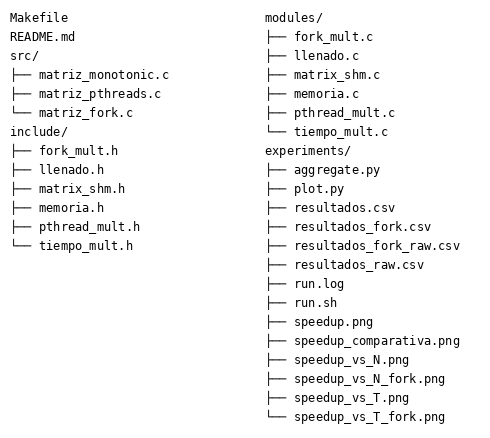
\includegraphics[width=0.95\textwidth]{figuras/estructura_proyecto.png}
    \caption{Estructura de carpetas y archivos del proyecto.}
    \label{fig:estructura}
\end{figure}

\subsection{Versión secuencial}

Es el programa base sobre el que se construyen las versiones paralelas. Recibe como argumentos el tamaño de la matriz \texttt{N} y un valor máximo, reserva memoria para tres matrices, las llena con números aleatorios, ejecuta el triple bucle de multiplicación y mide el tiempo. El código vive en \texttt{src/matriz\_monotonic.c}.

\subsection{Versión con pthreads}

Variante que reparte las filas de la matriz resultado entre varios hilos usando la API POSIX Threads. Los hilos se crean con \texttt{pthread\_create} y el programa principal espera con \texttt{pthread\_join}. El código de la paralelización vive en \texttt{modules/pthread\_mult.c}.

\subsection{Versión con fork y memoria compartida}

Variante que crea procesos con \texttt{fork()} en lugar de hilos. Como cada proceso tiene su propio espacio de direcciones, las matrices se crean en \textbf{memoria compartida POSIX} para que padre e hijos vean los mismos datos. El padre espera a cada hijo con \texttt{waitpid()}. El código de la paralelización vive en \texttt{modules/fork\_mult.c} y la gestión de la memoria compartida en \texttt{modules/matrix\_shm.c}.

\subsection{Estrategia de partición}

Las tres versiones paralelas usan la \textbf{misma estrategia}: repartir las filas de la matriz resultado $C$ entre los trabajadores. Cada uno calcula las filas que le corresponden y solo escribe en esa parte, así que no hay conflicto entre ellos.

El reparto es equitativo: si $N$ es divisible por la cantidad de hilos/procesos, cada uno recibe $N/T$ filas. Si no, los primeros reciben una fila extra para balancear la carga. El siguiente ejemplo muestra la partición para $N = 1000$ y $T = 4$:

\begin{center}
\begin{tabular}{|c|c|}
\hline
\textbf{Hilo / Proceso} & \textbf{Filas asignadas} \\
\hline
0 & $[0, 250)$ \\
1 & $[250, 500)$ \\
2 & $[500, 750)$ \\
3 & $[750, 1000)$ \\
\hline
\end{tabular}
\end{center}

\subsection{Por qué no se necesita sincronización adicional}

Como cada hilo o proceso escribe \textbf{exclusivamente} en su propio rango de filas de la matriz $C$, no hay condiciones de carrera: dos trabajadores nunca escriben sobre la misma posición. Los trabajadores leen de $A$ y $B$ sin escribir, lo cual es seguro. La única sincronización necesaria es al final: \texttt{pthread\_join} en la versión pthreads, o \texttt{waitpid} en la versión fork, para que el programa principal espere a que todos terminen antes de mostrar el resultado.

\section{Diseño experimental}

Esta sección describe cómo se diseñó el experimento. El profesor hizo énfasis en que el diseño experimental es la parte más importante del documento, porque sin un buen diseño los números no significan nada.

\subsection{Hardware}

Todas las mediciones se realizaron en el mismo equipo, por los integrantes del grupo. Las características son:

\begin{itemize}
    \item \textbf{CPU}: Intel Core i5-12450HX (12.\textsuperscript{a} generación).
    \item \textbf{Núcleos lógicos}: 12 (8 núcleos físicos con \textit{hyperthreading} activo).
    \item \textbf{Sistema operativo}: Linux.
    \item \textbf{Compilador}: \texttt{gcc} versión reciente con flags \texttt{-Wall -Wextra -O2}.
\end{itemize}

\subsection{Variables}

\begin{itemize}
    \item \textbf{Tamaño de la matriz} (\texttt{N}): 500, 1000, 2000, 4000 y 8000. Se eligió un rango amplio con saltos de factor 2 para cubrir tanto problemas chicos (donde el paralelismo es marginal) como problemas grandes (donde el paralelismo muestra todo su potencial).
    \item \textbf{Cantidad de hilos o procesos} (\texttt{T}): 1 (secuencial), 2, 4, 8 y 16. Para la versión fork se saltea \texttt{T=1} porque es esencialmente la misma versión secuencial que ya está medida.
    \item \textbf{Variable medida}: tiempo de la multiplicación en segundos, usando \texttt{clock\_gettime(CLOCK\_MONOTONIC\_RAW)}.
    \item \textbf{Métrica calculada}: \textit{speedup} = tiempo secuencial / tiempo paralelo.
\end{itemize}

En total se ejecutan \textbf{250 mediciones con pthreads} (5 tamaños × 5 configuraciones × 10 corridas) y \textbf{200 mediciones con fork} (5 × 4 × 10).

\subsection{Metodología: 10 corridas por configuración}

Para cada combinación de tamaño y cantidad de hilos/procesos se ejecutaron \textbf{10 corridas independientes} y se calculó la mediana, la media y la desviación estándar. El profesor insistió en que una sola medición no es confiable porque una sola corrida puede coincidir con un momento de ruido del sistema (otra tarea, una preempción, etc.). Repetir 10 veces y usar la mediana como estimador central reduce el impacto de esos picos.

Para la versión fork se midió el tiempo desde \textbf{antes del primer \texttt{fork()}} hasta \textbf{después del último \texttt{waitpid()}}. Es decir, se incluye el \textit{overhead} de crear y destruir procesos, igual que en la versión pthreads se incluye el \textit{overhead} de crear y juntar hilos. Esto permite comparar ambas técnicas en igualdad de condiciones. \textbf{antes del primer \texttt{fork()} hasta después del último \texttt{waitpid()}. Es decir, se incluye el \textit{overhead} de crear y destruir procesos, igual que en la versión pthreads se incluye el \textit{overhead} de crear y juntar hilos. Esto permite comparar ambas técnicas en igualdad de condiciones.

\subsection{Orden de los bucles}

El script que automatiza el experimento recorre las repeticiones por fuera y los tamaños por dentro:

\begin{verbatim}
for run_id in 1..10:
    for N in [500, 1000, 2000, 4000, 8000]:
        medir(N, T)
        sleep 1
\end{verbatim}

Es decir, para cada repetición se recorren todos los tamaños antes de pasar a la siguiente repetición. La razón, explicada por el profesor, es que si las 10 repeticiones de un mismo $N$ se hicieran seguidas, los datos quedarían \textit{calientes} en la caché del procesador y la medición saldría artificialmente rápida. Al intercalar tamaños se fuerza al sistema a traer datos nuevos de RAM, dando un resultado más realista.

\subsection{Automatización y resumibilidad}

Para no tener que ejecutar manualmente las 450 mediciones, se escribieron dos scripts:

\begin{itemize}
    \item \texttt{experiments/run.sh}: un script en bash que itera sobre las configuraciones, ejecuta cada medición y guarda el resultado en un CSV. Detecta si una medición ya está hecha y la saltea, por lo que si el proceso se interrumpe (Ctrl+C, corte de luz, etc.) se puede reanudar sin perder lo avanzado.
    \item \texttt{experiments/plot.py}: lee los CSV y genera las gráficas de speedup.
\end{itemize}

El experimento se ejecutó con el siguiente comando:

\begin{verbatim}
nohup bash experiments/run.sh > experiments/run.log 2>&1 &
\end{verbatim}

El \texttt{nohup} permite que el script siga corriendo aunque se cierre la terminal, y el \texttt{\&} lo deja en segundo plano. Las mediciones tardan entre algunas horas (N chicos) y varias horas (N=8000), por lo que es necesario dejarlo desatendido.

\section{Resultados}

En esta sección se muestran los tiempos medidos y los speedup calculados. Los valores que se reportan son la \textbf{mediana} de las 10 corridas, porque es la medida más robusta frente a valores atípicos. Todos los tiempos están en segundos.

\subsection{Tiempos medidos con pthreads}

La tabla~\ref{tab:tiempos-pthreads} muestra el tiempo de la multiplicación para la versión pthreads en segundos.

\begin{table}[ht]
\centering
\begin{tabular}{|c|r|r|r|r|r|}
\hline
\textbf{N} & \textbf{T=1} & \textbf{T=2} & \textbf{T=4} & \textbf{T=8} & \textbf{T=16} \\
\hline
500  & 0.044  & 0.101  & 0.053  & 0.034  & 0.032 \\
1000 & 0.423  & 0.753  & 0.398  & 0.266  & 0.204 \\
2000 & 4.36   & 7.12   & 3.76   & 2.39   & 1.64 \\
4000 & 75.65  & 68.22  & 40.30  & 29.68  & 24.29 \\
8000 & 2441.6 & 690.9  & 416.9  & 354.1  & 401.5 \\
\hline
\end{tabular}
\caption{Tiempos de ejecución con pthreads (segundos, mediana de 10 corridas).}
\label{tab:tiempos-pthreads}
\end{table}

\subsection{Tiempos medidos con fork}

La tabla~\ref{tab:tiempos-fork} muestra lo mismo para la versión fork. No se midió \texttt{T=1} porque es esencialmente la versión secuencial ya medida arriba.

\begin{table}[ht]
\centering
\begin{tabular}{|c|r|r|r|r|}
\hline
\textbf{N} & \textbf{T=2} & \textbf{T=4} & \textbf{T=8} & \textbf{T=16} \\
\hline
500  & 0.029  & 0.022  & 0.015  & 0.015 \\
1000 & 0.239  & 0.143  & 0.130  & 0.117 \\
2000 & 4.86   & 2.36   & 1.98   & 3.01 \\
4000 & 110.5  & 65.3   & 59.1   & 64.6 \\
8000 & 1197.2 & 742.7  & 796.2  & 940.1 \\
\hline
\end{tabular}
\caption{Tiempos de ejecución con fork (segundos, mediana de 10 corridas).}
\label{tab:tiempos-fork}
\end{table}

\subsection{Speedup con pthreads}

La tabla~\ref{tab:speedup-pthreads} muestra el \textit{speedup} de pthreads calculado como tiempo secuencial / tiempo paralelo.

\begin{table}[ht]
\centering
\begin{tabular}{|c|r|r|r|r|}
\hline
\textbf{N} & \textbf{T=2} & \textbf{T=4} & \textbf{T=8} & \textbf{T=16} \\
\hline
500  & 0.44 & 0.83 & 1.27 & 1.40 \\
1000 & 0.56 & 1.06 & 1.59 & 2.07 \\
2000 & 0.61 & 1.16 & 1.83 & 2.66 \\
4000 & 1.11 & 1.88 & 2.55 & 3.11 \\
8000 & 3.53 & 5.86 & 6.90 & 6.08 \\
\hline
\end{tabular}
\caption{Speedup de pthreads.}
\label{tab:speedup-pthreads}
\end{table}

\subsection{Speedup con fork}

La tabla~\ref{tab:speedup-fork} muestra el \textit{speedup} de fork. La base secuencial usada es la misma que para pthreads (\texttt{T=1} de la versión secuencial).

\begin{table}[ht]
\centering
\begin{tabular}{|c|r|r|r|r|}
\hline
\textbf{N} & \textbf{T=2} & \textbf{T=4} & \textbf{T=8} & \textbf{T=16} \\
\hline
500  & 1.54 & 1.99 & 2.89 & 2.88 \\
1000 & 1.77 & 2.95 & 3.25 & 3.62 \\
2000 & 0.90 & 1.85 & 2.20 & 1.45 \\
4000 & 0.69 & 1.16 & 1.28 & 1.17 \\
8000 & 2.04 & 3.29 & 3.07 & 2.60 \\
\hline
\end{tabular}
\caption{Speedup de fork (comparado con el T=1 de pthreads).}
\label{tab:speedup-fork}
\end{table}

\subsection{Comparativa pthreads vs fork}

La tabla~\ref{tab:comparativa} compara directamente las dos técnicas. La columna ``Mejor'' indica qué técnica dio mayor speedup en esa combinación.

\begin{table}[ht]
\centering
\small
\begin{tabular}{|c|c|c|c|c|}
\hline
\textbf{N} & \textbf{T} & \textbf{pthreads} & \textbf{fork} & \textbf{Mejor} \\
\hline
500  & 2  & 0.44 & 1.54 & fork \\
500  & 4  & 0.83 & 1.99 & fork \\
500  & 8  & 1.27 & 2.89 & fork \\
500  & 16 & 1.40 & 2.88 & fork \\
\hline
1000 & 2  & 0.56 & 1.77 & fork \\
1000 & 4  & 1.06 & 2.95 & fork \\
1000 & 8  & 1.59 & 3.25 & fork \\
1000 & 16 & 2.07 & 3.62 & fork \\
\hline
2000 & 2  & 0.61 & 0.90 & fork \\
2000 & 4  & 1.16 & 1.85 & fork \\
2000 & 8  & 1.83 & 2.20 & fork \\
2000 & 16 & 2.66 & 1.45 & pthreads \\
\hline
4000 & 2  & 1.11 & 0.69 & pthreads \\
4000 & 4  & 1.88 & 1.16 & pthreads \\
4000 & 8  & 2.55 & 1.28 & pthreads \\
4000 & 16 & 3.11 & 1.17 & pthreads \\
\hline
8000 & 2  & 3.53 & 2.04 & pthreads \\
8000 & 4  & 5.86 & 3.29 & pthreads \\
8000 & 8  & 6.90 & 3.07 & pthreads \\
8000 & 16 & 6.08 & 2.60 & pthreads \\
\hline
\end{tabular}
\caption{Comparativa de speedup: pthreads vs fork.}
\label{tab:comparativa}
\end{table}

\subsection{Gráficas}

La figura~\ref{fig:speedup-pt} muestra el speedup de la versión pthreads en función del tamaño de la matriz. Se observa que el speedup crece con $N$ y satura cerca de $N = 4000$.

\begin{figure}[ht]
    \centering
    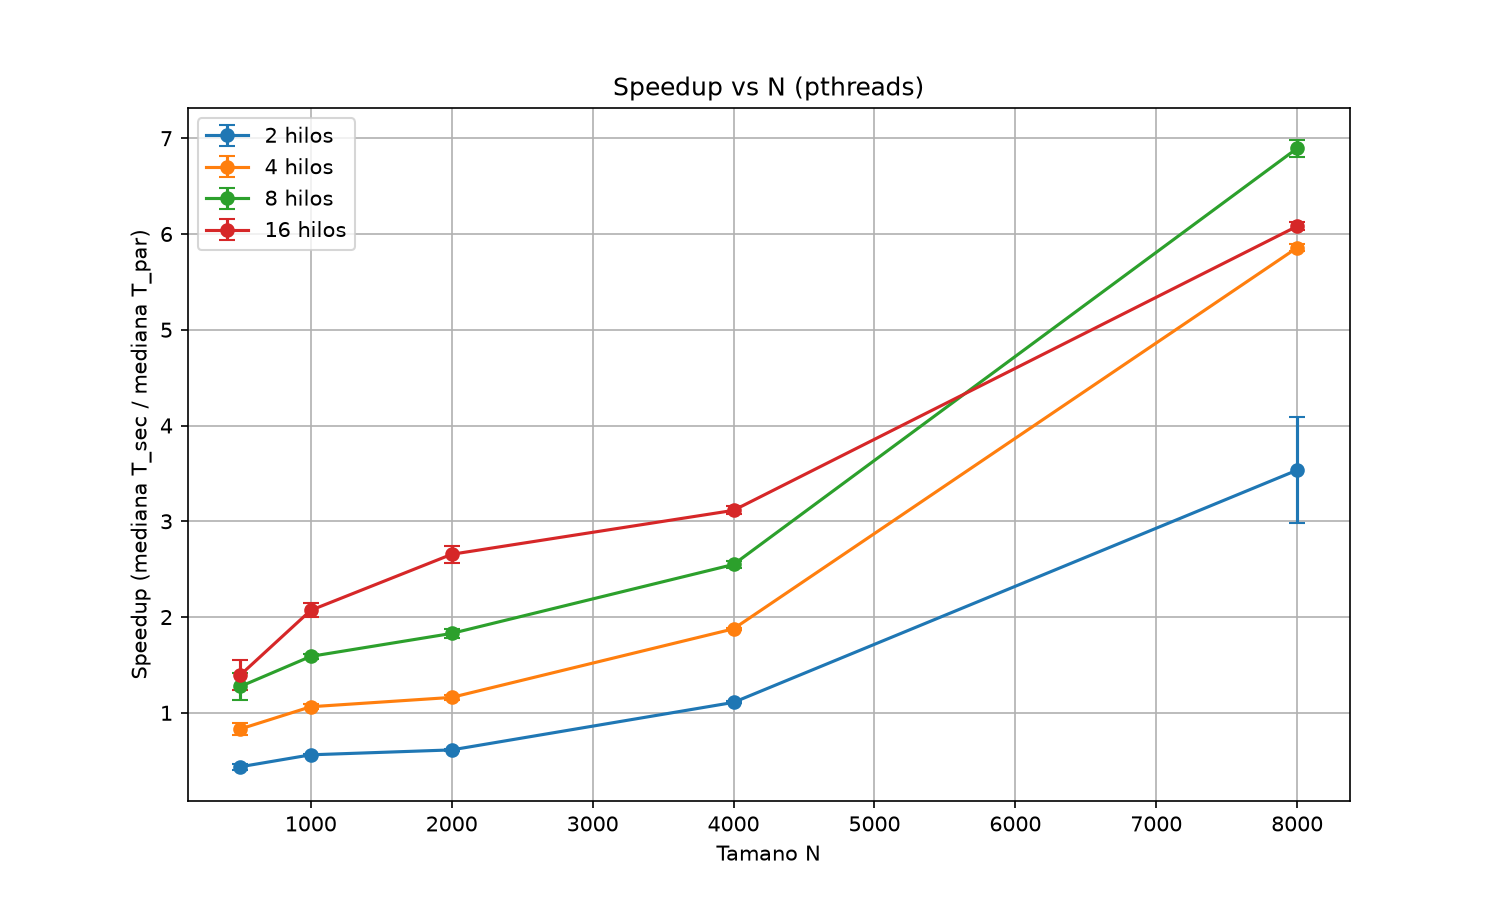
\includegraphics[width=0.85\textwidth]{figuras/speedup_vs_N.png}
    \caption{Speedup de pthreads en función del tamaño de la matriz. Cada curva representa una cantidad fija de hilos.}
    \label{fig:speedup-pt}
\end{figure}

La figura~\ref{fig:speedup-fork} muestra lo mismo para la versión fork. La forma es similar, pero los valores son diferentes: en $N$ chicos el speedup es más alto.

\begin{figure}[ht]
    \centering
    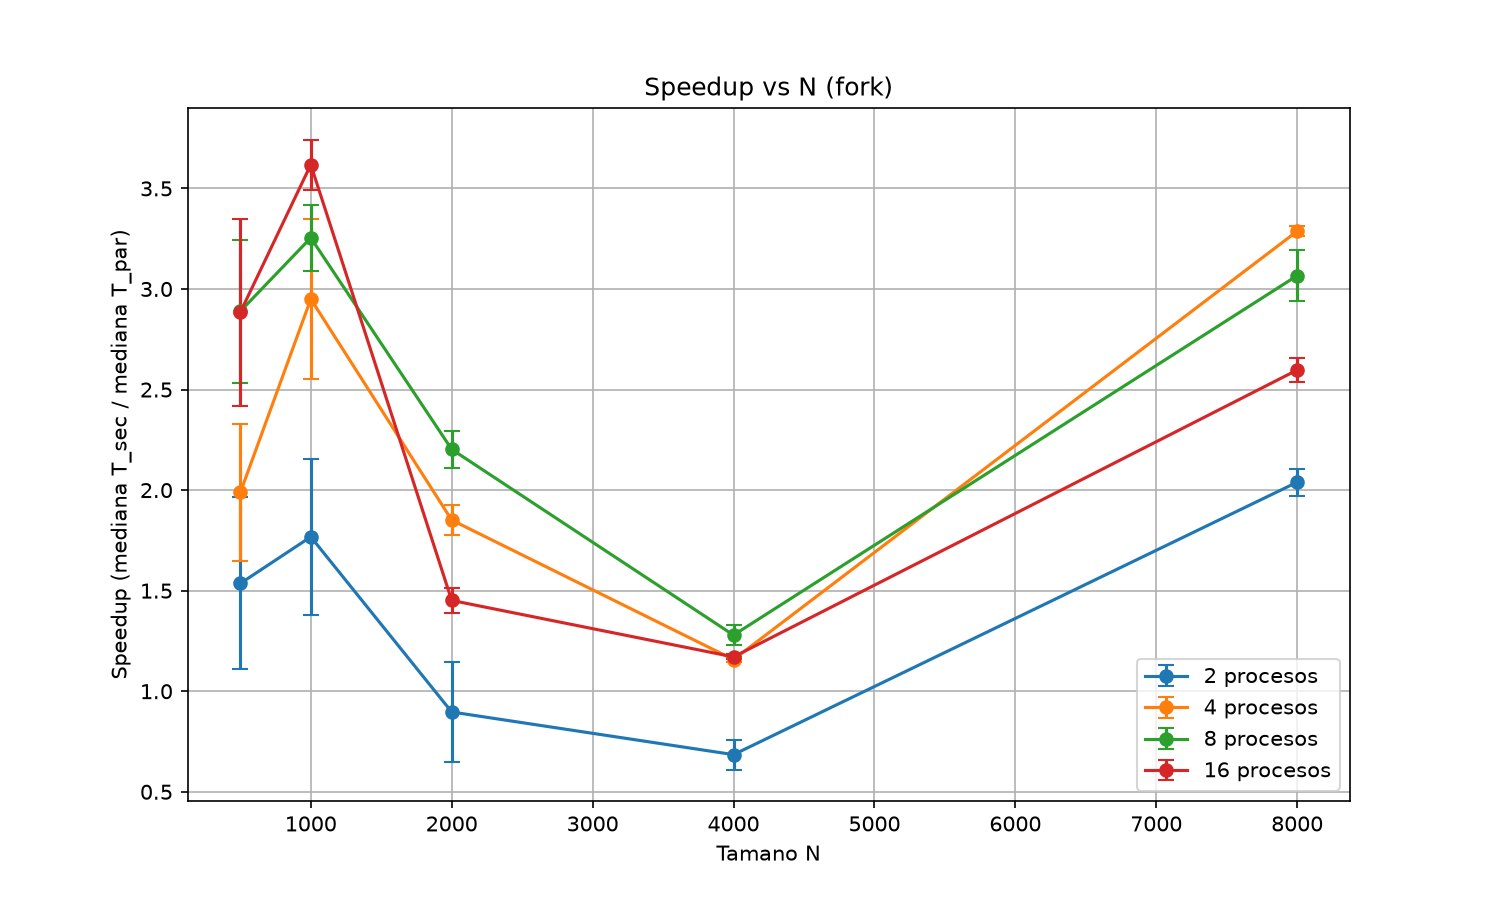
\includegraphics[width=0.85\textwidth]{figuras/speedup_vs_N_fork.png}
    \caption{Speedup de fork en función del tamaño de la matriz.}
    \label{fig:speedup-fork}
\end{figure}

La figura~\ref{fig:comparativa-plot} es la gráfica principal de este trabajo: muestra las 8 curvas (4 de pthreads y 4 de fork) en una sola imagen para facilitar la comparación directa.

\begin{figure}[ht]
    \centering
    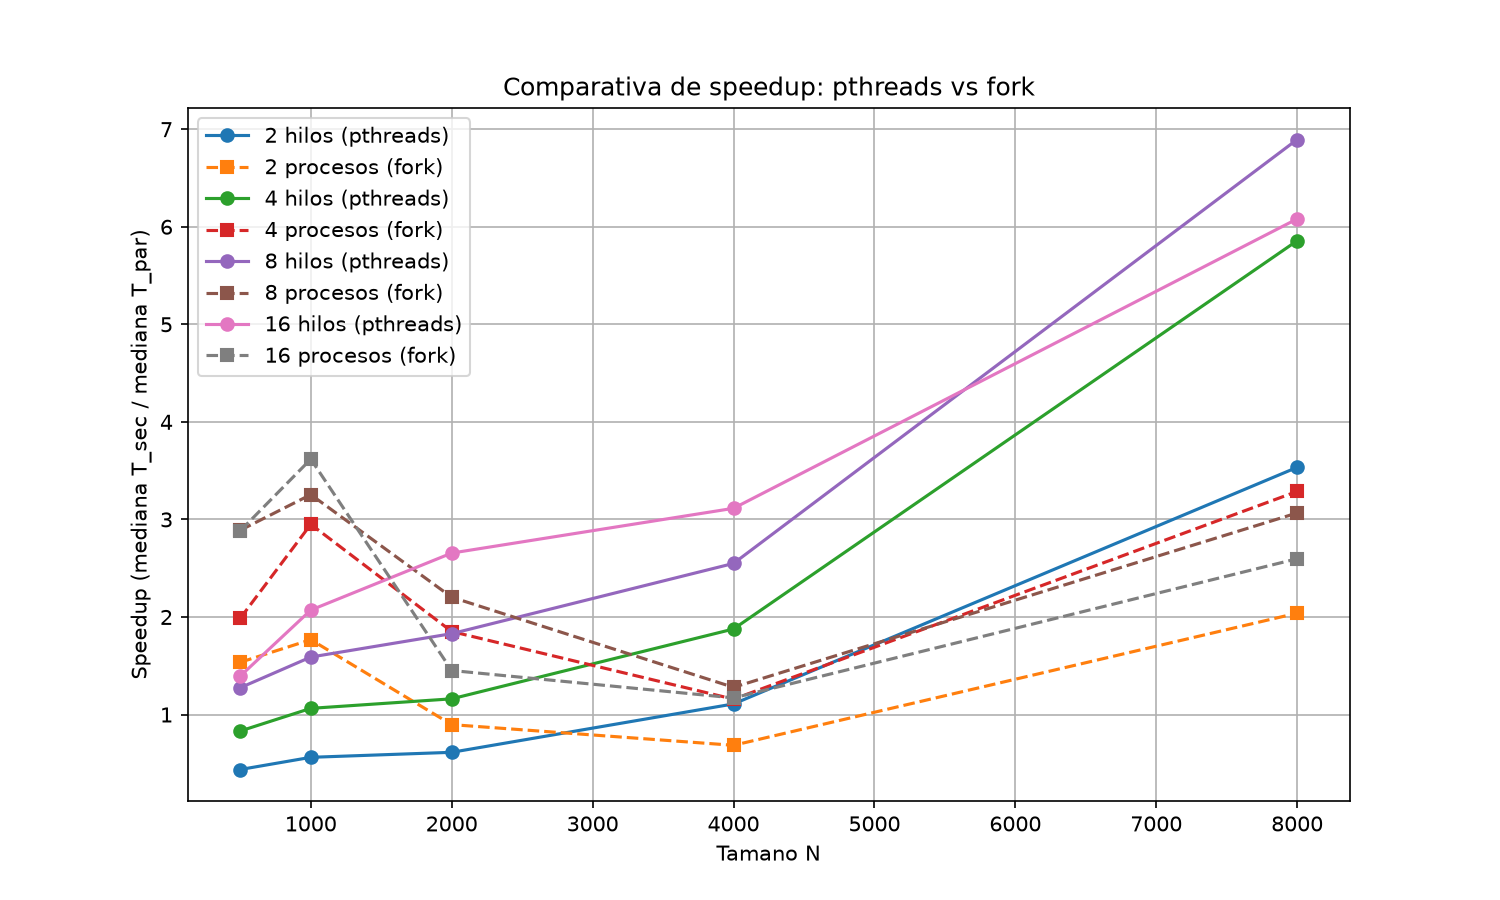
\includegraphics[width=0.85\textwidth]{figuras/speedup_comparativa.png}
    \caption{Comparativa de speedup: pthreads vs fork. Las líneas continuas con círculos son pthreads, las líneas punteadas con cuadrados son fork.}
    \label{fig:comparativa-plot}
\end{figure}

\subsection{Outliers detectados}

Al revisar las 10 corridas individuales de cada configuración con fork, se identificaron cinco valores atípicos puntuales. Todos corresponden a la \textbf{corrida número 10} de las configuraciones con $T = 2$. La tabla~\ref{tab:outliers} los resume.

\begin{table}[ht]
\centering
\begin{tabular}{|l|c|c|c|}
\hline
\textbf{Configuración} & \textbf{Outlier} & \textbf{Tiempo típico} & \textbf{Desviación} \\
\hline
N=500, T=2, run=10   & 0.057 s & $\sim$0.029 s & casi 2$\times$ \\
N=1000, T=2, run=10  & 0.426 s & $\sim$0.244 s & 80\% arriba \\
N=2000, T=2, run=10  & 9.84 s  & $\sim$4.86 s  & \textbf{el doble} \\
N=4000, T=2, run=10  & 152 s   & $\sim$110 s   & 37\% arriba \\
N=8000, T=2, run=10  & 1327 s  & $\sim$1197 s  & 11\% arriba \\
\hline
\end{tabular}
\caption{Valores atípicos puntuales en fork, todos en T=2 run=10.}
\label{tab:outliers}
\end{table}

Que todos los outliers caigan en la corrida 10 de las configuraciones con $T = 2$ sugiere que se debió a \textbf{ruido del sistema} en una ventana de tiempo específica (otra tarea puntual del sistema operativo), no a un problema del programa. El uso de la \textbf{mediana} como medida central hace que estos picos no distorsionen el speedup reportado, mientras que la media se vería fuertemente afectada.

\section{Análisis de resultados}

\subsection{Fork gana en problemas chicos}

En las matrices pequeñas ($N = 500$ y $N = 1000$), la versión con \texttt{fork()} supera claramente a la versión con pthreads. Por ejemplo, con $N = 1000$ y 16 procesos fork logra un speedup de 3.62$\times$, mientras que pthreads con 16 hilos solo llega a 2.07$\times$.

Esto puede sonar contra-intuitivo, porque crear un proceso es más caro que crear un hilo. La explicación está en que para problemas chicos, \textbf{el tiempo total es muy pequeño} y la mayor parte de lo que se mide es \textit{overhead}. El \textit{overhead} de fork (crear el proceso, esperar, limpiar) se paga una sola vez por medición, así que pesa menos proporcionalmente. En cambio, el \textit{overhead} de pthreads, aunque más liviano, se paga 16 veces (uno por cada hilo).

\subsection{Pthreads gana en problemas grandes}

En las matrices grandes ($N = 4000$ y $N = 8000$), la tendencia se invierte. Con $N = 8000$ y 8 hilos, pthreads alcanza un speedup de 6.90$\times$, mientras que fork con 8 procesos solo llega a 3.07$\times$: pthreads es más del doble de rápido.

La razón: cuando el problema es grande, el cómputo domina y el \textit{overhead} pesa menos. Ahí se ve el costo real de las dos estrategias:

\begin{itemize}
    \item \textbf{pthreads}: comparten memoria de forma \textbf{implícita}. No hay que configurar nada especial para que vean los mismos datos.
    \item \textbf{fork}: cada proceso tiene su propia imagen de memoria. Para compartir las matrices hay que pasar por \texttt{shm\_open}, \texttt{mmap} y \texttt{shm\_unlink}. Cuando $N$ es grande y los datos son grandes, ese trabajo extra de configuración se nota.
\end{itemize}

\subsection{El punto de cruce está en $N = 2000$}

Mirando la tabla~\ref{tab:comparativa} y la figura~\ref{fig:comparativa-plot}, se ve que en $N = 2000$ las dos técnicas están prácticamente empatadas: en algunas configuraciones gana fork y en otras gana pthreads. Este es el \textbf{punto de cruce} entre las dos técnicas. Para matrices más chicas que $N = 2000$ conviene fork; para matrices más grandes, conviene pthreads.

\subsection{Los outliers y la robustez de la mediana}

El patrón de los outliers (todos en T=2, run=10) muestra por qué fue importante repetir 10 veces y usar la mediana. Si solo se hubiera medido una vez por configuración, algunos speedup habrían sido pesimistas por culpa de ese ruido.

El contraste es claro: la media es sensible a un valor extremo, mientras que la mediana lo ignora. Por ejemplo, en $N = 2000$ con $T = 2$:

\begin{itemize}
    \item Media = 5.38 s
    \item Mediana = 4.86 s
    \item Diferencia = 11\% (el outlier de 9.84 s infla la media)
\end{itemize}

Si el speedup se hubiera calculado con la media, habría sido 3.28$\times$; con la mediana, 3.53$\times$. La diferencia no es dramática, pero confirma que la mediana es la elección correcta.

\section{Conclusiones}

\subsection{Logros del trabajo}

Se cumplió el objetivo general del caso de estudio: se implementaron dos versiones paralelas del programa de multiplicación de matrices, una con \textbf{POSIX Threads} y otra con \textbf{procesos + memoria compartida POSIX}, y se compararon con la versión secuencial usando la métrica estándar de speedup.

El diseño experimental fue riguroso: 10 corridas por configuración, 5 tamaños de matriz, hasta 5 cantidades de hilos/procesos, en total 450 mediciones. El script se diseñó de forma que se puede pausar y reanudar sin perder datos, lo cual fue clave para un experimento de varias horas.

\subsection{Hallazgos principales}

\begin{enumerate}
    \item \textbf{No hay una técnica universalmente mejor}: la elección entre pthreads y fork depende del tamaño del problema. En este equipo, para matrices chicas ($N < 2000$) fork fue mejor; para matrices grandes ($N \geq 4000$) pthreads fue mejor.
    \item \textbf{El speedup real está lejos del ideal}. El mejor caso fue 6.90$\times$ con 8 hilos en $N = 8000$, mientras que el ideal sería 8$\times$ con 8 hilos o 12$\times$ con 12 procesos (recordando que la máquina tiene 12 núcleos lógicos). La diferencia se debe a la parte secuencial del programa, la contención por memoria y el \textit{overhead} del sistema.
    \item \textbf{Repetir el experimento 10 veces y usar la mediana fue clave}: se detectaron outliers puntuales debidos a ruido del sistema, y la mediana los ignoró de forma natural.
    \item \textbf{El orden de los bucles en el script}: alternar tamaños entre repeticiones evitó que los datos se quedaran ``calientes'' en la caché del procesador, dando mediciones más realistas.
\end{enumerate}

\subsection{Limitaciones}

\begin{itemize}
    \item El speedup de fork se calculó contra el $T = 1$ de \textbf{pthreads} (no se midió fork $T = 1$ por separado). En teoría fork $T = 1$ debería dar un tiempo similar al secuencial de pthreads, pero no se verificó experimentalmente.
    \item La versión fork con $N = 8000$ usa mucha memoria: tres matrices de 256\,MB cada una, más la imagen del proceso. En máquinas con menos RAM podría fallar.
    \item El experimento se hizo en un solo equipo. En otra máquina con distinto hardware (más o menos núcleos, diferente jerarquía de caché) los resultados podrían cambiar.
\end{itemize}

\subsection{Trabajo futuro}

Como continuación natural de este trabajo se podrían explorar:

\begin{itemize}
    \item Implementar la versión con procesos midiendo también \texttt{T=1}, para tener un baseline propio de fork.
    \item Probar tamaños de matriz aún más grandes ($N = 16000$ o más) para ver si la tendencia de pthreads ganando se mantiene.
    \item Aplicar optimizaciones al algoritmo (caché blocking, orden de los bucles cambiado) y medir cómo afectan al speedup.
    \item Probar en una máquina con muchos más núcleos (32 o 64) para ver hasta dónde escala cada técnica.
\end{itemize}


\section{Referencias}
\begin{itemize}
    \item \textbf{The Open Group Base Specifications Issue 7 (POSIX.1-2008)} — \texttt{pthread\_create}, \texttt{pthread\_join}, \texttt{fork()}, \texttt{waitpid()}, \texttt{shm\_open}, \texttt{mmap}, \texttt{clock\_gettime}. Documentación oficial de la API POSIX utilizada en este trabajo.
    \item \textbf{GNU C Library (glibc) Manual} — Documentación de las funciones de la biblioteca estándar de C, incluyendo la implementación de pthreads y memoria compartida en sistemas Linux.
    \item \textbf{Material del curso de Computación de Alto Rendimiento} — Presentaciones y grabaciones de clase utilizadas como referencia conceptual (wall clock vs tiempo de CPU, 10 corridas, orden de los bucles, quantum, memoria compartida).
\end{itemize}


\end{document}
